\documentclass[
a4paper,
12pt,
oneside,
headsepline,		% Linie für Kopfzeile
footsepline,		% Linie für Fußzeile
%bibtotoc
]{scrbook}
 
% Druckbereich: \areaset[BCOR]{textwidth}{textheight}
% BCOR ist "Binding Correction", also wieviel Innenrand verloren geht
% A4 hat 297mm x 210mm
% wenn keine Marginalien, dann ist Breite 15cm vielleicht besser
% \areaset[1.5cm]{14cm}{25cm}
 \usepackage[left=3cm,right=2cm,bottom=2.5cm]{geometry}
%% Die folgende Zeile sorgt dafür, daß die Fußnoten eingerückt werden,
%% und zwar um 2em (class scrbook).
\deffootnote{2em}{2em}{\textsuperscript{\normalfont\thefootnotemark} }
 
\usepackage[utf8x]{inputenc}  % Unterstützung für Unicode-Zeichen-Eingabe
\usepackage[T1]{fontenc}      % Unterstützung für Europäische-Zeichen-Ausgabe
\usepackage{ae}               % verbesserte Unterstützung für Umlaute
\usepackage[german]{babel}    % deutsche Übersetzungen und Wortumbrüche
\usepackage[scaled]{helvet}  % schönere Schriftart: Helvetica
\usepackage{mathptmx}            % passende Mathe-Schriftart
\usepackage{courier}             % passende Monospaced-Schriftart
\usepackage{pgf}              % Unterstützung für Graphiken
\usepackage{tikz}             % Unterstützung für Graphiken
\usepackage[onehalfspacing]{setspace}
\usepackage{acronym} 
\usepackage{listings}
\usepackage{color}
\usepackage{float}

\definecolor{Gray}{gray}{0.9}
\definecolor{sun1}{rgb}{0.2,0.2,0.4}
\definecolor{sun2}{rgb}{0.4,0.4,0.6}
\definecolor{sun3}{rgb}{0.6,0.6,0.8}
\definecolor{sun4}{rgb}{0.8,0.8,1}
\definecolor{msblau}{rgb}{0.31,0.4,0.517}
\definecolor{darkred}{rgb}{0.5,0,0}
\definecolor{darkgreen}{rgb}{0,0.5,0}
\definecolor{darkblue}{rgb}{0,0,0.5}
 
\usepackage[                
   pdftex,                  % Ausgabe-Medium: PDF
   colorlinks=true,         % farbige Links in der Bildschirm-Version?
   pdfstartview=FitV,       % wie soll Acrobat starten?
   linkcolor=blue,         % Farbe für Querverweise
   citecolor=blue,         % Farbe für Zitierungen
   urlcolor=blue,          % Farbe für Links
   bookmarks=true
   ]{hyperref}              % Paket für Links im PDF
 
%%%% Informationen über den Text festlegen %%%%%%%%%%%%%%%%%%%%%%%%%%%%%%%%%%
\title{Bachelorarbeit}
\author{Andreas Collmann}
\date{\today}
 
%%% hier können noch viel viel mehr Einstellungen kommen
%%%% hier beginnt der Inhalt %%%%%%%%%%%%%%%%%%%%%%%%%%%%%%%%%%%%%%%%%%%%%%%%
%\spacing{1.5}

\makeindex

\newcommand{\eruck}[1]{
    \noindent\hspace*{#1}
}
\newcommand{\zab}[1]{
    \vspace*{#1}
}
\newcommand{\fina}[1]{
    {\em #1}
}
\newcommand{\finar}[1]{
    {\fina{#1}\textsuperscript{\textregistered}}		
}
\newcommand{\sona}[1]{
    {\em #1}
}
\newcommand{\code}[1]{
    {\\ \eruck{20mm} \texttt{#1} \\}
}

% Formatierung Quellcode

\lstset{
    language=Python,
	numbers=left,
    breaklines=true,
	backgroundcolor=\color{Gray},
	basicstyle=\small,
	showspaces=false,
    basicstyle=\scriptsize\ttfamily,
    keywordstyle=\bfseries\ttfamily\color{orange},
    stringstyle=\color{blue}\ttfamily,
    commentstyle=\color{gray}\ttfamily,
    emph={square}, 
    emphstyle=\color{blue}\texttt,
    emph={[2]root,base},
    emphstyle={[2]\color{orange}\texttt},
    showstringspaces=false,
    flexiblecolumns=false,
    tabsize=2,
    numbers=left,
    numberstyle=\tiny,
    numberblanklines=false,
    stepnumber=1,
    numbersep=10pt,
    xleftmargin=15pt
	}

\begin{document}

 %\section*{}
%\newpage
%\addtocounter{page}{-1}
 
 %%%%%%%%%%%%%%%%%%%%%%%%%%%            Titelseite           %%%%%%%%%%%%%%%%%%%%%%%%%%%%%%%%%%%%%
\begin{titlepage}
 	  \centering
 		\begin{figure}[h]
 			\centering
 				\includegraphics[width=0.45\textwidth]{pic/h_da.png}
 			%\caption{innoQ \\ Robert-Bosch-Straße 7 \\ 64293 Darmstadt}
 			\label{fig:innoq}
 		\end{figure}	 
 		\zab {2cm}
 		\textbf{\Large Hochschule Darmstadt} \\		 
 		\zab {0,4cm}
 		{\Large - Fachbereich Informatik -} \\ 		 
 		\zab {3cm}
 		{\large Untersuchung der Offenen Schnittstellen des Ur5 Roboters anhand eines Anwendungsbeispiels} \\
 		\zab {2cm}
 		Abschlussarbeit zur Erlangung des akademischen Grades Bachelor of Science
 		(B.Sc.)  \\	 
 		\zab {1cm}
 		vorgelegt von \\
 		\zab {1cm}
 		{\Large Andreas Collmann} \\ 
 		\zab {2cm}
 		\begin{tabular}{ll}
 		    Referent: & Prof. Dr. Horsch\\
 		    Korreferent: & Prof. Dr. Akelbein\\
 		\end{tabular}
\end{titlepage}
 
 \include{doc/erklaerung}
 \section*{Abstract}
\label{abstract}

Um die Vorteile des kollaborativen Arbeitens von Menschen und Robotern anzuwenden, wird im Zuge dieser Arbeit der für die Kollaboration zugelassene Roboter UR5 der Firma ``Universal Robots'' untersucht. Es wird untersucht, welche Möglichkeiten diesen Roboter zu programmieren möglich sind. Die Untersuchung erfolgt aufgrund einiger Kriterien, die auf den Einsatz mit Kollaboration zielen.
Die Schnittstellen des UR5 Roboters werden untersucht und dokumentiert.
Am Ende dieser Arbeit wird eine Entscheidungsfindung zusammengefasst, welche Schnittstelle zu welchem Anwendungsfall am besten zu wählen ist. Um dies zu evaluieren, wurde eine Beispielanwendung in jeder Schnittstelle entwickelt. Die Ergebnisse sind am Ende knapp zusammengefasst.
 
 \tableofcontents
 \listoffigures
 \listoftables
 \lstlistoflistings
 
 \chapter{Einleitung}
\label{einleitung}

\section{Fachliche Umgebung}
\label{fachliche_domaene}

In der Industrie werden Roboter in den Fertigungsanlagen eingesetzt. 
Dies geschieht meist nur in Koordination mit anderen Robotern, jedoch nie kollaborativ mit Menschen. In der Nähe dieser Roboter darf sich kein Mensch aufhalten. Die Roboter sind umhaust, sprich in einem speziellen Bereich abgesichert, damit keine Unfälle passieren können. 
Auf diese Weise kann man sehr effizient über automatisierte Fließbandstraßen Produkte herstellen. 
Bisher gibt es nur wenig Roboter, die entsprechende Sicherheitsauflagen erfüllen, um mit Menschen zu kollaborieren.

\section{Motivation und Ziel des Projekts}
\label{projektziel_motivation}

Industrieroboter unterstützen die Produktion von Produkten, jedoch zumeist noch in abgesicherten Bereichen. Wenn eine sehr filigrane Arbeit gefragt ist, muss das Werkstück von einem Menschen bearbeitet werden, da der Mensch wesentlich bessere Fähigkeiten hat, auf Probleme zu reagieren oder Korrekturen vorzunehmen. In diesem Fall wird die Produktion unterbrochen. Das Produkt muss aus dem umhausten Bereich gebracht werden, wo es von einem Menschen bearbeitet werden kann.
\\
Für die Prodution wäre es viel sinnvoller und zeitsparender, wenn Roboter für den Menschen so sicher sind, dass keine Trennung zwischen Mensch und Robotern existiert.
\\\\
In vielen Arbeitsbereichen wie z. B. Pflege und Medizin, müssen oft Hebe-Arbeiten ausgeführt werden. Dies führt dazu, dass die Menschen in solchen Berufen im späteren Alltag mit Rückenproblemen oder ähnlichem Leiden leben müssen. Roboter, die eingesetzt werden, um diese Lasten abzunehmen, würden die Arbeit erleichtern und Verletzungen vorbeugen.
\\\\
Es soll untersucht werden, inwiefern es möglich ist, den UR5 Roboter zu programmieren, um mit Menschen zu kollaborieren.

\section{Aufgabenstellung}
\label{aufgabenstellung}

Der UR5 Roboter besitzt mehrere Programmierschnittstellen. Für diese Schnittstellen soll ein Anwendungsprogramm erstell werden.
Dieses Anwendungsprogramm soll als eine Beispielanwendung einer Roboter-Mensch Kollaboration dienen.
Diese verschiedenen Programme werden miteinander verglichen. Es soll eine Entscheidungshilfe gegeben werden, für welchen Anwendungsfall welche Schnittstelle am besten geeignet ist. Hierfür werden Kriterien erhoben, die auf die Beispielanwendung zugeschnitten sind.
Menschen wollen Eingaben nicht wiederholen, deshalb sollen erhobene Daten persistent gespeichert werden.

\section{Einordnung in die Themenfelder der Informatik}
\label{sec:einordnung}

Die Schnittstellen werden mit den etablierten Programmiersprachen C/C++ und Python programmiert. Hinzu kommt noch die eigens von Universal Robots entwickelte URScript Sprache.
Da auch versucht wird, den Roboter von einem anderen Rechner zu steuern, wird auch Netzwerkprogrammierung benötigt.
Für die Steuerung des Roboters wird auf das Themenfeld Robotik eingegangen. Robotik ist nicht in den Grundlagen für den Bachelor-Studiengang der Informatik enthalten, deswegen sind die Themenfelder dieser Arbeit etwas weiter gestreut.
 \chapter{Grundlagen}

\section{Roboter-Mensch-Kollaboration}
\label{sec:roboter-mensch-kollaboration_gru}

Man unterscheidet die Arbeiten mit einem Roboter unter mehrere Arten.
Roboter die mit anderen Robotern gleichzeitig arbeiten nennt man Kooperation zwichen Robotern.
Der Mensch ist in diesem Arbeitsumfeld nicht dabei und kann nur von außen einfluss nehmen.
\\\\
Als nächstes gibt es die Kollaboration zwichen dem Roboter und dem Mensch. 
Hier wird auch eine Unterteilung vorgenommen die unterschiedliche Richtlinien erfordern.

\begin{itemize}
\item Sicherhaltshalt, wenn der Mensch den Kollaborationsraum betritt.
\item Dauerhafte Überwachung des Abstands zwichen Mensch und Roboter, der mit reduzierter Geschwindigkeit arbeitet.
\item Verminderte Geschwindigeit. Führung des Roboters durch den Mensch. Sensoren erfassen die Kräfte, die vom Menschen ausgeführt werden und übertragen sie auf den Roboter.
\item Beschränkung der im Roboter ausgeführten Energie. Überwachung des Roboters auf Kollision und sofortigem Stop
\end{itemize}

\subsection{Richtlinien}
\label{kol_richtlinien_gru}

In so gut wie allen fällen sind Roboter in der Industrie in einem extra abgesicherten Bereich umzäunt, damit kein Arbeiter sich verletzen kann. Diese Robote sind umhaust. Es ist nicht möglich in einem gemeinsamen Arbeitsbereich zu kollaborieren. 
Damit Menschen im Arbeitsbereich vom Robotern Arbeiten dürfen müssen diese Roboter bestimmte Sicherheitsrichtlinien entsprechen.
Der Roboter darf unter keinen Umständen eine Lebensbedrohliche gefahr darstellen. Die Norm \ac{ISO} 10218

\section{UR5 Roboter}
\label{sec:ur_robot_gru}

Die Dänische Firma Universal Robots hat den leichten UR5 und mittelgroßen UR10 Roboter hergestellt mit den erfüllbaren Normen, um mit diesem Roboter zu kollaborieren. Man kann sich im laufenden Betrieb in der Nähe aufhalten um Wegpunkte zu Teachen oder auch gleichzeitig an einem Werkstück zu arbeiten. 
Im Folgenden Kapitel werden die Eigenschaften des UR5 Roboters erörtert.

\subsection{Kinematik}
\label{ur_eigenschaften_gru}

\begin{figure}[ht]
  \centering
    \includegraphics[width=0.8\textwidth]{pic/ur5_robot.png}
      \caption[UR5 Roboter]{Abbildung zeigt den UR5 Roboter von universal Robots}
      \label{fig:schnittstellen_schichten}
\end{figure}

Der Roboter besitzt 6 Gelenke die ihm ermöglichen einen 360° Arbeitsbereich mit einem Radius von ca 85cm zu ermöglichen. Gesteuert wird er von einem Linux Rechner, der sich in der Nähe befindet. 
Die Festplatte für das System ist eine Speicherkarte, die leicht ausgetauscht werden kann.
\\\\
Um den Rechner anzusprechen existiert bei lieferung ein Touch Tablet, das für das Linux System den Visuellen Output gibt. bei Start wird auch automatisch die Software für den Roboter gestartet. Die Software nennt sich Polyscope und wurde in Java geschrieben. Diese Software verbindet sich per TCP/IP auf den \ref{URControl}. Ein Server Programm das die Schnittstelle von dem Linux System zu dem Roboter Controller auf dem Rechner Herstellt.
\\\\
Die Polyscope Software läuft im normalen Modus und den Administrativen Modus. Der Normale Modus ermöglicht es Programme zu erstellen, laufen zu lassen und Grundeinstellungen vorzunehmen. Außerdem kann ein Software Update der Polyscope Software gemacht werden.

\subsection{Peripherie}
\label{ur_update_gru}

Zwei Arten von Updates sind hier zu unterscheiden. Zum einen kann das Linux System geupdatet werden. Auf normalem wege über den Packetmanager des Systems, oder wenn man das neuste Image von Universal Robots runterläd und dann das System neu aufspielt. Hier ist jedoch zu beachten, dass dabei alle Daten verloren gegangen werden. Deshalb sollte eine Datensicherung vorgenommen werden. Wie dies geschieht wird im darauf folgenden Unterkapitel beschrieben(\ref{ur_datensicherung_gru}).
\\\\
Updates für dem Roboter müssen allerdings manuell gemacht werden. Hierfür müssen die aktuellen Updates von der Homepage von Universal Robots runtergeladen werden. Die Update-Datei muss mit der dateiendung .urup auf einen USB Stick mit einem FAT32 Dateisystem abgelegt werden.\\\\
Nachdem der USB Stick an das Linuy System angeschlossen ist, kann von der Polyscope Software das Update ausgeführt werden. Einstellungen->Updates.\\
Im Administrativen Modus können nach dem Update die Firmware's der einzelnen Gelenkcontroller geupdatet werden. Die werden im Update mitgeliefert. Die einzelnen Schritte sind in den Dokumentationen beiliegend auf der CD zu finden.

\subsection{Datensicherung}
\label{ur_datensicherung_gru}

Die Daten des Roboters sind abgelegt in root verzeichniss unter 

\begin{lstlisting}[caption={Pfade Der Ur5 Relevanten Dateien}, label=lst:ur5data ,captionpos=b] 
/root/.urcontrol    #Konfigurationsdateien des Ur5Roboters
/programs   		#alle geschriebenen Programme unter Polyscope
\end{lstlisting}

Es ist möglich die Dateien per USB Stick zu sichern oder über Programme wie ``SCP'' über das Netzwerk zu Kopieren.

\section{Programmierschnittstellen vom UR5}
\label{sec:programm_api_uebersicht_gru}

Der Ur5 Roboter kann auf drei Ebenen angesprochen werden.\\

\begin{itemize}
\item Polyscope
\item URscript
\item C-Api
\end{itemize}

\begin{figure}[ht]
  \centering
    \includegraphics[width=0.8\textwidth]{pic/ur_programming_levels.png}
      \caption[Schichten der Software Schnittstellen]{Übersicht über die
      Schichten der bestehenden Software Schnittstellen des Ur5 Roboters}
      \label{fig:schnittstellen_schichten}
\end{figure}

\section{Kriterien für die Bewertung der Schnittstellen}
\label{sec:criterias_of_solutions_kon}

Die Schnittstellen werden wie folgt bewertet:

\begin{itemize}
\item Programmierbarkeit
\item Interaktion mit Programm,
\item Möglichkeit zu Debuggen und Testbarkeit
\item Aufwendung
\end{itemize}

Wie schwer ist es ein Programm für die einzelnen Schnittsellen zu entwickeln.
Kann der Mensch das Programm Intuitiv bedienen? Wichtig hierbei ist, dass der Mensch mit dem Roboter Kommunizieren kann. Dies geschieht am besten, wenn der Mensch nicht Kryptisch was eingeben muss. Der Mensch braucht Anwenderfreundliche Programme.
\\\\
Beim Entwickeln von Programmen ist es wichtig, dass der Entwickler Fehler im Programm entdeckt um diese schnell zu beheben.
Je Größer und Komplexer das Programm wird, desto schwieriger wird es Fehler zu entdecken.

\section{URControl}
\label{sec:ur_control_gru}

Der URController eine Server Anwendung die auf dem Rechner des Roboters läuft. 
Dieser Controller dient als Schnittstelle von der Roboter Hardware und der Software die den Roboter ansteuern wollen.

\subsection{Konfiguration des URControllers}
\label{urcontrol_rci_gru}

Den URController kann man bevor er gestartet wird in einer Konfigurationsdatei konfigurieren.
Hier werden wichtige Einstellungen vorgenommen, die zu den jeweiligen Modellen der Ur5 oder Ur10 Serie gehören. Folgend ist ein ausschnitt der Konfigurationsdatei zu sehen
\\
\begin{lstlisting}[caption={Ausschnitt aus der Datei urcontrol.conf zur vorkonfigurierung des UR5 Roboters}, label=lst:ur5_conf ,captionpos=b]
[Config]
# masterboard_version, 0 = Zero-series, 1 = One-series, 
# 3 = Pause function enabled, 4 = first cb2 version, 5 = ur10 support added
masterboard_version = 4
dump_bytecode_on_exception = 1

[Hardware]
controller_box_type = 2 # 1=CB1, 2=CB2UR5, 3=CB2UR10
robot_type = 1  # 1=UR5, 2=UR10
robot_sub_type = 1
\end{lstlisting}

\subsection{Echtzeit Schnittstelle}
\label{urcontrol_rci_gru}

Die Echtzeit Schnittstelle ist eine TCP Schnittstelle, die im 125Hz Takt Nachrichten an die Clients sendet. Diese Schnittstelle empfängt keine Daten von den Clients. Diese Nachrichten müssen von den Clients analysiert und zerlegt werden. Die Daten werden in einer bestimmten form gesendet

TODO !! listing echtzeit schnittstelle

Die Client Anwendung muss nun dieses Packet \ac{parsen}
Wie Die einzelnen Packete aussehen sind im Anhang mitgeliefert
Für die Programmiersprache C wurde ein ein Parser dafür geschrieben.

\subsection{Secondary und Primary Schnittstelle}
\label{urcontrol_spi_gru}

Das Secondary Interface ist eine \ac{TCP/IP} Schnittstelle, die in einem 60Hz Takt Nachrichten über den Roboter an Verbundene Rechner sendet.
Die Nachrichten beinhalten Informationen wie z.B. den Roboter Status, die Positionen der einzelenen Joints.
Die volle Beschreibung welche Informationen gesendet werden ist im anhang zu finden.

Zusätzlich, kann die Secondary Schnittstelle Befehle von Verbundenen Rechnern empfangen. 
Diese Befehle können URScript befehle sein. Ein ganzes Programm aus URScript befehlen oder spezielle zugelassene Befehle die den Roboter Status verändern.

\begin{figure}[ht]
  \centering
    \includegraphics[width=0.5\textwidth]{pic/secondary_datapackage_scheme.png}
      \caption[Schema des Datenpackets gesendet von der Secondary Schnittstelle]{Grobe Darstellung wie das Nachrichten Packet gesendet von der Secondary/Primary Schnittstelle.}
      \label{fig:datascheme_of_secondary_interface}
\end{figure}

\subsection{Polyscope}
\label{urcontrol_polyscope_gru}

Polyscope ist eine Anwendung die auf dem Roboter-Rechner läuft. Die Anwendung verbindet sich per \ac{TCP/IP} auf den URControl(\ref{sec:ur_control_gru}) und sendet URScript befehler an den Roboter um diesen zu steuern.
Diese Anwendung wird auf dem Tablet angezeigt. Hierrüber kann man per Touch eingabe ein neues \ac{URP} Programm erstellen. Dieses Programm wird zur Laufzeit in ein Script umgewandelt. Die Polyscope Software schickt nun in Schritten die einzelnen Scriptbefehle an den URControl, der diese ausführt. Im Programmbaum kann eingesehen werden an welchem Schritt das Programm sich befindet.

\section{C-API}
\label{sec:rest_prinzip_gru}

Die C-\ac{API} ist von dem Hersteller \ac{UR} eine zur Verfügung gestellte C \ac{Library} mit einer Header Datei, die etwaige Funktionen der Library erklärt. Die Header Datei enthält nicht alle Funktionen, somit sind nicht alle zugänglich. Die C-\ac{API} erlaubt es einen eigenen Controller für den Roboter zu entwickeln. Der für den Roboter zur Verfügung gestellte Controller mit der Polyscope Software und eine anwendung die, die C-\ac{API} benutzt, kann aber nicht gleichzeitig laufen. Es schließen sich also die Programmiersprache URScript  und ein eigener Controller zunächst aus. Es könnte ein eigener Controller entwickelt werden, der die Befehle in URScript selbst interpretiert und diese wie bei dem URControll ausführt. So könnte man die vorhandene Sprache nehmen und diese sogar erweitern.

\subsection{Kontrollstruktur}
\label{capi_control_loop_gru}	

Die C-\ac{API} ermöglicht es eine Verbindung zum Roboter zu öffnen und über eigene Funktionen Befehle abzuschicken. Dies erfolgt in einem streng festgelegten Muster.

\begin{lstlisting}[language=C,caption={Beispiel der Kontroll Struktur}, label=lst:robot_control_loop,captionpos=b]
  while(!endcondition) { // At ROBOT_CONTROLLER_FREQUENCY times per second
    robotinterface_read_robot_state_blocking();
    robotinterface_get_actual_positions(&positions);
     // >>> various calculations <<<
    robotinterface_command_position_velocity_acceleration( xxx, yyy, zzz);
    robotinterface_send_robot_command();
  }
\end{lstlisting}

die Funktion robotinterface\_read\_state\_blocking() startet den Bereich in dem Datenabfragen an den Roboter gestellt werden können. Daten wie zb. Temperatur der Motoren, der Stand der Gelenke, die Geschwindigkeit der Gelenke, etc. in der Dokumentation beiliegend zu dieser Arbeit sind alle Daten noch einmal aufgelistet. Nachdem die Daten abgefragt wurden, kann mit C-\ac{API} Functionen Position, Geschwindigkeit und Beschleunigungswerte übermittelt werden, die der Roboter durch seinen Regler auszuführen versucht.\\
Es können jedoch keine Wegpunkte festgelegt werden, die dann automatisch vom Roboter angefahren werden. Dies muss der Entwickler selbst 
berechnen. Es gibt mehrere Verfahren, in dieser Arbeit sind \ac{PTP}-Verfahren und Linear Verfarhen(siehe Kapitel \ref{bewegungsprofile_gru}) getestet worden. In der beiliegenden Dokumentation ist aufgeführt wie man dies möglicherweise berwerkstelligen könnte.
\\\\
Zum Abschluss wird die Function robotinterface\_send() aufgerufen die dafür sorgt, dass der Acht Millisekundentakt eingehalten wird und die Befehle an den Roboter weiterleitet. Falls die Acht Millisekunden überschritten werden, wird der Roboter in einen Sicherheitsmodus gesetzt
und der Roboter wird angehalten.\\
Wenn so etwas im UR-Kontroller passiert, kann der Anwender diese wieder abschalten wenn alles in Ordnung ist. Dies muss mit der C-\ac{API} selbst geschrieben werden. Die C-\ac{API} liefert hierfür auch Funktionen. Das die richtigen Richtlinien aber auch eingehalten werden, muss von dem Wechsel des Sicherheitsmodus in den normalen Modus eine Benutzerabfrage verlangt werden.

\subsection{Bewegungsprofile}
\label{bewegungsprofile_gru}

\ac{PTP} Verfahren 

Um den Roboter bestimmten Wegpunkten abfahren zu lassen, muss man die Bewegungsprofile selbst berechnen und ǘber die C-API an den Roboter im 125Hz Takt übergeben. Das PTP Verfahren setzt dabei vorraus das die einzelnen Positionen der Gelenke bekannt sind. Der Wert ist angegeben in radiant. Die Zielposition

Linear Verfahren

Das Lineare Verfahren bedeutet eine Bewegung des Roboters von dem TCP Punkt aus. Sie verfährt Linear, bedeutet das die Orientierung 
des TCP Punktes sich nicht ändert. Da in diesem Verfahren die Berechnung der Position des TCP Punktes verwendet wird, ist es nötig die Position des TCP im Raum zu kennen um eine Strecke zu einem Ziel Punkt abfahren zu können. Der Roboter kann aber nur Positionen die der Sechs Gelenke verarbeiten. Es muss also eine umrechnung stattfinden. Diese umrechung wird Inverse Kinematic genannt. Die Berechnung für die Ineverse Kinematic ist von einem anderen Projekt entnommen worden.
 \chapter{Evaluierungskonzept}
\label{konzept_kon}

\section{Anwendungsbeispiel}
\label{sec:anwendung_kon}

Das Anwendungsbeispiel ist ein Kinderspiel. Dieses Spiel soll die motorischen Fähigkeiten bei Kindern verbessern.
Gegeben ist ein Kugel mit löschern aus Verschiedenen Formen(Kreis, Oval, Viereck, Trapez, etc.). Zu diesen Formen existieren die Entsprechenden Klötzchen, die entsprechend Groß sind un die Form der Löscher besitzen. Die Aufgabe des Spiel ist es alle Klötzchen in die entsprechende Form zu drücken, bis alle in der Kugel sind.

\begin{figure}[H]
  \centering
    \includegraphics[width=0.6\textwidth]{pic/ur5_robot.png}
      \caption[Kinder Geschicklichkeitsspiel]{Kinderspiel zur Evaluierung der Software Schnittstellen}
      \label{fig:kinderspiel}
\end{figure}

Die Kugel wird an den Kopf des Roboterarms befestigt. Es soll eine Anwendung entwickelt werden, die für den entsprechenden Spieler die Höhe des Roboters einstellt. Der Spieler soll die Möglichkeit haben, die Startposition zu verstellen und für sich zu speichern. Bei einem bestimmten Knopf druck soll der Roboter das Loch für die jeweils nächste Form so ausrichten, damit der Mensch das Klötzchen nur noch einwerfen braucht.

\section{Speichern der Anwendungsdaten}
\label{sec:save_of_data_kon}

Um auf bestimmte Menschen zugeschnittene Bewegungsabläufe zu machen muss der Roboter Daten über den Anwender kennen. Diese sollten persistent gespeichert werden, damit bei einem Wechsel des Anwenders die Daten nicht verloren gehen.
Daten der Anwender sind z.B. Name, Alter, bestimmte Positionen im Roboter Programm, etc.
\\\\
\textbf{Speichern über Polyscope und URScript}
\label{sec:save_data_polyscope_kon}
\\\\
In der Polyscope Software oder in einem URScript Programm, können Daten die von den Benutzern erstellt oder erhoben werden nicht persistent
gespeichert werden. Hierzu muss eine zweite Anwendung entwickelt werden, auf die sich das URScript oder \ac{URP} Programm verbindet und die Daten zum persistenten speichern versendet.
In Polyscope und URScript muss sehr aufwendig mit den vorhandenen Script Befehlen eine Socket Verbindung aufgebaut werden.
Damit diese zwei Programme miteinander Kommunizieren können muss ein gemeinsames Protokoll mit bestimmten Befehlen festgelegt werden. Es ist möglich Text, Zahlen oder Dezimalzahlen zu versenden und zu empfangen. Es kann nur eins dieser drei Typen versendet, von dem aber beliebig viele. 
\\\\
\textbf{Speichern über Eigene API}
\label{save_data_own_api_kon}
\\\\
Mit der Eigenen API muss keine zweite Software entwickelt werden, da die API auf einem Client Rechner läuft und dort die Daten persistent gespeichert werden können. Es muss im Anwendungsprogramm eine Verbindung zu einer Datenbank aufgebaut werden und dort können die Daten gespeichert werden.
 \chapter{Realisierung}
\label{chap:umsetzung}

\section{TCP Server mit Datenbank zum dauerhaften speichern der Daten}
\label{sec:tcp_datentank_sicherung_rel}

Um mit Polyscope und URScript erhobene Daten zu Speichern wurde ein kleiner TCP Server geschrieben, der eine verbindung zulässt und Daten in einer Datenbank Speichert. Die Daten sind Objectorientiert, und werden von dem Server erstellt. 
In Polyscope und URScript gibt es keine Objectorientierung, deshalb musss dort alles nacheinander angefragt werden. 

\section{C-API}
\label{sec:capi_rel}
Lorem ipsum dolor sit amet, consetetur sadipscing elitr, sed diam nonumy eirmod tempor invidunt ut labore et dolore magna aliquyam erat, sed diam voluptua. At vero eos et accusam et justo duo dolores et ea rebum. Stet clita kasd gubergren, no sea takimata sanctus est Lorem ipsum dolor sit amet. Lorem ipsum dolor sit amet, consetetur sadipscing elitr, sed diam nonumy eirmod tempor invidunt ut labore et dolore magna aliquyam erat, sed diam voluptua. At vero eos et accusam et justo duo dolores et ea rebum. Stet clita kasd gubergren, no sea takimata sanctus est Lorem ipsum dolor sit amet.


\subsection{gelöste Aufgabe}
\label{sub:capi-problems_rel}
Lorem ipsum dolor sit amet, consetetur sadipscing elitr, sed diam nonumy eirmod tempor invidunt ut labore et dolore magna aliquyam erat, sed diam voluptua. At vero eos et accusam et justo duo dolores et ea rebum. Stet clita kasd gubergren, no sea takimata sanctus est Lorem ipsum dolor sit amet. Lorem ipsum dolor sit amet, consetetur sadipscing elitr, sed diam nonumy eirmod tempor invidunt ut labore et dolore magna aliquyam erat, sed diam voluptua. At vero eos et accusam et justo duo dolores et ea rebum. Stet clita kasd gubergren, no sea takimata sanctus est Lorem ipsum dolor sit amet.


\subsection{Aufgetretene Probleme}
\label{sub:capi-problems_rel}
Lorem ipsum dolor sit amet, consetetur sadipscing elitr, sed diam nonumy eirmod tempor invidunt ut labore et dolore magna aliquyam erat, sed diam voluptua. At vero eos et accusam et justo duo dolores et ea rebum. Stet clita kasd gubergren, no sea takimata sanctus est Lorem ipsum dolor sit amet. Lorem ipsum dolor sit amet, consetetur sadipscing elitr, sed diam nonumy eirmod tempor invidunt ut labore et dolore magna aliquyam erat, sed diam voluptua. At vero eos et accusam et justo duo dolores et ea rebum. Stet clita kasd gubergren, no sea takimata sanctus est Lorem ipsum dolor sit amet.


\section{Polyscope}
\label{sec:Polyscope_rel}

\subsection{Programmierung}
\label{programmierung_polyscope_rel}
Lorem ipsum dolor sit amet, consetetur sadipscing elitr, sed diam nonumy eirmod tempor invidunt ut labore et dolore magna aliquyam erat, sed diam voluptua. At vero eos et accusam et justo duo dolores et ea rebum. Stet clita kasd gubergren, no sea takimata sanctus est Lorem ipsum dolor sit amet. Lorem ipsum dolor sit amet, consetetur sadipscing elitr, sed diam nonumy eirmod tempor invidunt ut labore et dolore magna aliquyam erat, sed diam voluptua. At vero eos et accusam et justo duo dolores et ea rebum. Stet clita kasd gubergren, no sea takimata sanctus est Lorem ipsum dolor sit amet.


\subsection{Benutzer Interaktion}
\label{user_interaktion_polyscope_rel}
Lorem ipsum dolor sit amet, consetetur sadipscing elitr, sed diam nonumy eirmod tempor invidunt ut labore et dolore magna aliquyam erat, sed diam voluptua. At vero eos et accusam et justo duo dolores et ea rebum. Stet clita kasd gubergren, no sea takimata sanctus est Lorem ipsum dolor sit amet. Lorem ipsum dolor sit amet, consetetur sadipscing elitr, sed diam nonumy eirmod tempor invidunt ut labore et dolore magna aliquyam erat, sed diam voluptua. At vero eos et accusam et justo duo dolores et ea rebum. Stet clita kasd gubergren, no sea takimata sanctus est Lorem ipsum dolor sit amet.

\subsection{Test und Fehlersuche im Programm}
\label{debuggin_polyscope_rel}
Bevor Polyscope ein Programm ablaufen lässt wird das Script auf die richtige Syntax geprüft. Sollte ein Fehler vorhanden sein wird dies beim Start als Popup angezeigt. Fehler die in Abschnitten mit Touch hinzugefügt wurden, können jedoch nicht lokalisiert werden. Nur in extra eingefügtem Script code kann grob lokalisiert werden, was für ein Fehler aufgetreten ist, weil dieser Teil extra geprüft wird.

\subsection{Aufwand der Programmierung}
\label{polyscope_aufwand}
Lorem ipsum dolor sit amet, consetetur sadipscing elitr, sed diam nonumy eirmod tempor invidunt ut labore et dolore magna aliquyam erat, sed diam voluptua. At vero eos et accusam et justo duo dolores et ea rebum. Stet clita kasd gubergren, no sea takimata sanctus est Lorem ipsum dolor sit amet. Lorem ipsum dolor sit amet, consetetur sadipscing elitr, sed diam nonumy eirmod tempor invidunt ut labore et dolore magna aliquyam erat, sed diam voluptua. At vero eos et accusam et justo duo dolores et ea rebum. Stet clita kasd gubergren, no sea takimata sanctus est Lorem ipsum dolor sit amet.

\section{URScript}
\label{sec:ur_script_rel}
Lorem ipsum dolor sit amet, consetetur sadipscing elitr, sed diam nonumy eirmod tempor invidunt ut labore et dolore magna aliquyam erat, sed diam voluptua. At vero eos et accusam et justo duo dolores et ea rebum. Stet clita kasd gubergren, no sea takimata sanctus est Lorem ipsum dolor sit amet. Lorem ipsum dolor sit amet, consetetur sadipscing elitr, sed diam nonumy eirmod tempor invidunt ut labore et dolore magna aliquyam erat, sed diam voluptua. At vero eos et accusam et justo duo dolores et ea rebum. Stet clita kasd gubergren, no sea takimata sanctus est Lorem ipsum dolor sit amet.

\subsection{Laden des Scripts auf den Controller}
\label{load_script_rel}
Lorem ipsum dolor sit amet, consetetur sadipscing elitr, sed diam nonumy eirmod tempor invidunt ut labore et dolore magna aliquyam erat, sed diam voluptua. At vero eos et accusam et justo duo dolores et ea rebum. Stet clita kasd gubergren, no sea takimata sanctus est Lorem ipsum dolor sit amet. Lorem ipsum dolor sit amet, consetetur sadipscing elitr, sed diam nonumy eirmod tempor invidunt ut labore et dolore magna aliquyam erat, sed diam voluptua. At vero eos et accusam et justo duo dolores et ea rebum. Stet clita kasd gubergren, no sea takimata sanctus est Lorem ipsum dolor sit amet.

\subsection{Programmierung}
\label{programmierung_ur_script_rel}
Lorem ipsum dolor sit amet, consetetur sadipscing elitr, sed diam nonumy eirmod tempor invidunt ut labore et dolore magna aliquyam erat, sed diam voluptua. At vero eos et accusam et justo duo dolores et ea rebum. Stet clita kasd gubergren, no sea takimata sanctus est Lorem ipsum dolor sit amet. Lorem ipsum dolor sit amet, consetetur sadipscing elitr, sed diam nonumy eirmod tempor invidunt ut labore et dolore magna aliquyam erat, sed diam voluptua. At vero eos et accusam et justo duo dolores et ea rebum. Stet clita kasd gubergren, no sea takimata sanctus est Lorem ipsum dolor sit amet.

\subsection{Test und Fehlersuche im Programm}
\label{ur_script_debuggen}
Lorem ipsum dolor sit amet, consetetur sadipscing elitr, sed diam nonumy eirmod tempor invidunt ut labore et dolore magna aliquyam erat, sed diam voluptua. At vero eos et accusam et justo duo dolores et ea rebum. Stet clita kasd gubergren, no sea takimata sanctus est Lorem ipsum dolor sit amet. Lorem ipsum dolor sit amet, consetetur sadipscing elitr, sed diam nonumy eirmod tempor invidunt ut labore et dolore magna aliquyam erat, sed diam voluptua. At vero eos et accusam et justo duo dolores et ea rebum. Stet clita kasd gubergren, no sea takimata sanctus est Lorem ipsum dolor sit amet.

\subsection{Benutzer Interaktion}
\label{ur_script_user_interaction}
Lorem ipsum dolor sit amet, consetetur sadipscing elitr, sed diam nonumy eirmod tempor invidunt ut labore et dolore magna aliquyam erat, sed diam voluptua. At vero eos et accusam et justo duo dolores et ea rebum. Stet clita kasd gubergren, no sea takimata sanctus est Lorem ipsum dolor sit amet. Lorem ipsum dolor sit amet, consetetur sadipscing elitr, sed diam nonumy eirmod tempor invidunt ut labore et dolore magna aliquyam erat, sed diam voluptua. At vero eos et accusam et justo duo dolores et ea rebum. Stet clita kasd gubergren, no sea takimata sanctus est Lorem ipsum dolor sit amet.

\subsection{Aufwand der Programmierung}
\label{ur_script_aufwand}

\section{Anwendung mit Eigener API}
\label{sec:script_hoerherer_schicht_rel}
Lorem ipsum dolor sit amet, consetetur sadipscing elitr, sed diam nonumy eirmod tempor invidunt ut labore et dolore magna aliquyam erat, sed diam voluptua. At vero eos et accusam et justo duo dolores et ea rebum. Stet clita kasd gubergren, no sea takimata sanctus est Lorem ipsum dolor sit amet. Lorem ipsum dolor sit amet, consetetur sadipscing elitr, sed diam nonumy eirmod tempor invidunt ut labore et dolore magna aliquyam erat, sed diam voluptua. At vero eos et accusam et justo duo dolores et ea rebum. Stet clita kasd gubergren, no sea takimata sanctus est Lorem ipsum dolor sit amet.

\subsection{Adapter zur Secondary Schnittstelle}
\label{beschreibung_script_hoeher_schicht}
Lorem ipsum dolor sit amet, consetetur sadipscing elitr, sed diam nonumy eirmod tempor invidunt ut labore et dolore magna aliquyam erat, sed diam voluptua. At vero eos et accusam et justo duo dolores et ea rebum. Stet clita kasd gubergren, no sea takimata sanctus est Lorem ipsum dolor sit amet. Lorem ipsum dolor sit amet, consetetur sadipscing elitr, sed diam nonumy eirmod tempor invidunt ut labore et dolore magna aliquyam erat, sed diam voluptua. At vero eos et accusam et justo duo dolores et ea rebum. Stet clita kasd gubergren, no sea takimata sanctus est Lorem ipsum dolor sit amet.

\subsection{Programmierung mit Adapter}
\label{programmierung_mit_hoerherer_schicht}
Lorem ipsum dolor sit amet, consetetur sadipscing elitr, sed diam nonumy eirmod tempor invidunt ut labore et dolore magna aliquyam erat, sed diam voluptua. At vero eos et accusam et justo duo dolores et ea rebum. Stet clita kasd gubergren, no sea takimata sanctus est Lorem ipsum dolor sit amet. Lorem ipsum dolor sit amet, consetetur sadipscing elitr, sed diam nonumy eirmod tempor invidunt ut labore et dolore magna aliquyam erat, sed diam voluptua. At vero eos et accusam et justo duo dolores et ea rebum. Stet clita kasd gubergren, no sea takimata sanctus est Lorem ipsum dolor sit amet.

\subsection{Benutzer Interaktion}
\label{user_interaktion_mit_hoerherer_schicht}

Lorem ipsum dolor sit amet, consetetur sadipscing elitr, sed diam nonumy eirmod tempor invidunt ut labore et dolore magna aliquyam erat, sed diam voluptua. At vero eos et accusam et justo duo dolores et ea rebum. Stet clita kasd gubergren, no sea takimata sanctus est Lorem ipsum dolor sit amet. Lorem ipsum dolor sit amet, consetetur sadipscing elitr, sed diam nonumy eirmod tempor invidunt ut labore et dolore magna aliquyam erat, sed diam voluptua. At vero eos et accusam et justo duo dolores et ea rebum. Stet clita kasd gubergren, no sea takimata sanctus est Lorem ipsum dolor sit amet.

\subsection{Test und Fehlersuche im Programm}
\label{debuggen_mit_hoeherer schicht}
Lorem ipsum dolor sit amet, consetetur sadipscing elitr, sed diam nonumy eirmod tempor invidunt ut labore et dolore magna aliquyam erat, sed diam voluptua. At vero eos et accusam et justo duo dolores et ea rebum. Stet clita kasd gubergren, no sea takimata sanctus est Lorem ipsum dolor sit amet. Lorem ipsum dolor sit amet, consetetur sadipscing elitr, sed diam nonumy eirmod tempor invidunt ut labore et dolore magna aliquyam erat, sed diam voluptua. At vero eos et accusam et justo duo dolores et ea rebum. Stet clita kasd gubergren, no sea takimata sanctus est Lorem ipsum dolor sit amet.

\subsection{Aufwand der Programmierung}
\label{eigene_api_aufwand}
 \chapter{Ergebnis}
\label{sec:ErreichteErgebnisse}

Im Folgenden Kapitel werden die Schnittstellen gegenübergestellt und verglichen. Desweiteren werden die nicht erreichten Ziele erörtert.
\\\\
\begin{tabular}{|l|p{0.333\textwidth}|p{0.333\textwidth}|}
	\hline
	\textbf{Kriterium} & \textbf{C-API} & \textbf{Polyscope} 
	\\ \hline \hline 
	Programmierbarkeit & Schon für einfache Roboterprogramme ist es schwer zu programmieren & Leichter Einstieg zum Programmieren für Anfänger
	\\ \hline
	Benutzerinteraktion &  Es ist möglich ein übersichtliches \& intuitives Interface zu entwickeln & 
	Keine komplexen Menüs möglich/ Nur schwache Interaktion möglich.
	\\ \hline
	Testen & Tests sind möglich, aber nur mit Simulation des Roboters & Keine eigenen Tests möglich/ Getestet wird immer Live an Roboter.
	\\ \hline
	Debuggen & Compiler findet Syntax Fehler \& Debugging ist nur mit simuliertem Roboter möglich & Beim Testen live am Roboter, bedingt möglich.
	\\ \hline
	Aufwand & Sehr großer Aufwand von nöten/ Es muss alles selbst entwickelt werden. & \label{krit_polyscope_aufwand}
	Bei kleinen Programmen kaum Aufwand/ Aufwand steigt enorm bei mehr Anforderungen.\\ \hline
\end{tabular}
\captionof{table}{Zusammenfassung der Evaluierungskriterien für C-API und Polyscope}
\label{tab:vgl_interfaces_first}

\begin{tabular}{|l|p{0.33\textwidth}|p{0.33\textwidth}|}
	\hline
	\textbf{Kriterium} & \textbf{URScript} & \textbf{Eigener Adapter}\\ \hline \hline 
	Programmierung & Verständliche Dokumentation ermöglicht einen schnellen Einstieg/ Entwicklerwerkzeuge und Syntax Highlighting erleichtern die Übersicht und vereinfachen die Programmierung & eine etablierte Programmiersprache und vorhandene Software Bibliotheken erleichtern das Programmieren. \\
	\hline 
	Benutzerinteraktion & Die Möglichkeiten bleiben wie bei Polyscope auf Popups beschränkt(siehe \ref{user_interaktion_polyscope_rel}) & Wie bei C-API können \ac{GUI}s erstellt werden, die komplexe Formulare und Menüs bieten \\
	\hline 
	Testen & Mit gegebenen Mitteln sind automatische Tests nicht möglich. Es kann nur wie mit Polyscope Live getestet werden. & Automatische Tests sind möglich \\
	\hline
	Debuggen & Keine Möglichkeit zu Debuggen/ URController liefert bei Fehler in der Syntax keine Information & Fehler werden leicht gefunden, da die etablierten Programmiersprachen den Programmcode nach Syntaxfehlern durchsuchen und anzeigen
	\\
	\hline 
	Aufwand & Ähnlich wie bei Polyscope, jedoch etwas besser durch mehr Übersicht des Projekts & Anfangs ein großer Aufwand von Nöten. Bei mehreren Anwendungen für den Roboter ist Aufwand jedoch geringer als bei den anderen Schnittstellen.\\
	\hline 
\end{tabular}
\captionof{table}{Zusammenfassung der Evaluierungskriterien für URScript und eigenem Adapter}
\label{tab:vgl_interfaces_second}

\section{Vergleich der Schnittstellen}

\textbf{Die C-API} ist eine sehr hardwarenahe Schnittstelle zum Roboter. Der Aufwand, der betrieben werden muss ist äußerst hoch. Diese Schnittstelle sollte nur in seltenen Fällen eingesetzt werden. Nur spezielle Anwendungen, die wärend der Laufzeit Anpassungen an die Bewegungssteuerung geben, sollten diese Schnittstelle nutzen.
\newpage
\textbf{Die Polyscope Software} eignet sich hervorragend für wenige komplexe Anwendungen, die keine bzw. kaum Benutzerinteraktion erfordern. Für eine Kollaboration die auf direkte Kommunikation zwischen Mensch und Roboter angewiesen ist, ist diese Schnittstelle nicht zu empfehlen, denn diese sie kann nur sehr aufwändig auf persistente Daten zugreifen und speichern.
\\\\
\textbf{URScript} bietet in Sachen Benutzerinteraktion nur die gleichen Möglichkeiten wie die Polyscope Software(siehe \ref{ur_script_user_interaction}). Es ist übersichtlicher und verständlicher gegenüber Polyscope-Anwendungen zu entwickeln, bietet jedoch die eigens entwickelte Scriptsprache nur wenig Spielraum, um wirklich komplexe Anwendungen zu entwickeln.
\\\\
\textbf{Ein eigener Adapter} zum URController vereint die Vorteile einer etablierten Programmiersprache, nämlich vorhandene Entwicklerwerkzeuge und Software-Bibliotheken zu nutzen. Der Roboter wird über URScriptbefehle gesteuert, deshalb muss nicht tief in die Robotersteuerung, wie bei der C-API eingreifen werden. Wenn viel Benutzerinteraktion notwendig ist, ist diese Schnittstelle empfehlenswert.

\section{Nicht erreichte Ziele}
\label{sec:Nicht_erreichte_ziele}

Die aufgetretenen Probleme mit der C-API haben verhindert, dass keine vollständige Anwendung geschrieben werden konnte. Aus Zeitmangel wurde dort die Entwicklung abgebrochen. 
Die Fehler konnten ein wenig eingegrenzt werden. Ein Hardwaredefekt ist nicht auszuschließen. 
\\
Es ist nicht bekannt, welche C-API Version in dem URController benutzt wird. Die selbst erstellten Bewegungsprofile sehen korrekt aus, jedoch konnte man sehen, dass der URController funktionierende Soll-Werte übergeben hat. Es ist möglich, dass dem URController mehr Funktionen in der C-API zur Verfügung stehen.
 \chapter{Fazit}

\section{Ausblick}
\label{sec:ausblick}

\ref{sec:Nicht_erreichte_ziele} zu erreichen.

\section{Zusammenfassung}
\label{sec:Zusammenfassung}
Lorem ipsum dolor sit amet, consetetur sadipscing elitr, sed diam nonumy eirmod tempor invidunt ut labore et dolore magna aliquyam erat, sed diam voluptua. At vero eos et accusam et justo duo dolores et ea rebum. Stet clita kasd gubergren, no sea takimata sanctus est Lorem ipsum dolor sit amet. Lorem ipsum dolor sit amet, consetetur sadipscing elitr, sed diam nonumy eirmod tempor invidunt ut labore et dolore magna aliquyam erat, sed diam voluptua. At vero eos et accusam et justo duo dolores et ea rebum. Stet clita kasd gubergren, no sea takimata sanctus est Lorem ipsum dolor sit amet.

\subsection{C-API}
\label{sec:Zusammenfassung}
Lorem ipsum dolor sit amet, consetetur sadipscing elitr, sed diam nonumy eirmod tempor invidunt ut labore et dolore magna aliquyam erat, sed diam voluptua. At vero eos et accusam et justo duo dolores et ea rebum. Stet clita kasd gubergren, no sea takimata sanctus est Lorem ipsum dolor sit amet. Lorem ipsum dolor sit amet, consetetur sadipscing elitr, sed diam nonumy eirmod tempor invidunt ut labore et dolore magna aliquyam erat, sed diam voluptua. At vero eos et accusam et justo duo dolores et ea rebum. Stet clita kasd gubergren, no sea takimata sanctus est Lorem ipsum dolor sit amet.

\subsection{UR-Script}
\label{sec:Zusammenfassung}
Lorem ipsum dolor sit amet, consetetur sadipscing elitr, sed diam nonumy eirmod tempor invidunt ut labore et dolore magna aliquyam erat, sed diam voluptua. At vero eos et accusam et justo duo dolores et ea rebum. Stet clita kasd gubergren, no sea takimata sanctus est Lorem ipsum dolor sit amet. Lorem ipsum dolor sit amet, consetetur sadipscing elitr, sed diam nonumy eirmod tempor invidunt ut labore et dolore magna aliquyam erat, sed diam voluptua. At vero eos et accusam et justo duo dolores et ea rebum. Stet clita kasd gubergren, no sea takimata sanctus est Lorem ipsum dolor sit amet.
\subsection{Polyscope}
\label{sec:Zusammenfassung}
Lorem ipsum dolor sit amet, consetetur sadipscing elitr, sed diam nonumy eirmod tempor invidunt ut labore et dolore magna aliquyam erat, sed diam voluptua. At vero eos et accusam et justo duo dolores et ea rebum. Stet clita kasd gubergren, no sea takimata sanctus est Lorem ipsum dolor sit amet. Lorem ipsum dolor sit amet, consetetur sadipscing elitr, sed diam nonumy eirmod tempor invidunt ut labore et dolore magna aliquyam erat, sed diam voluptua. At vero eos et accusam et justo duo dolores et ea rebum. Stet clita kasd gubergren, no sea takimata sanctus est Lorem ipsum dolor sit amet.

 
 \clearpage
 \appendix
 
 \begin{thebibliography}{XXXXXX-JJJJa}

\bibliography{Literatur/quellen}

\renewcommand{\bibname}{A. ~Literaturverzeichnis}
\addcontentsline{toc}{chapter}{\protect\numberline{A}{Literaturverzeichnis}}
\setcounter{chapter}{1}

%\addcontentsline{toc}{chapter}{A. ~Literaturverzeichnis}

%\bibitem [DJAN-2013]: Organisation/Hersteller/Autor: Titel [: Untertitel].
%\url{URL}, [Datum, sofern auf Web-Seite angegeben], zuletzt besucht am Datum.
%(Internet)

\bibitem [DJAN-2013]: Name1, Vorname1[; Name2, Vorname2; ...]: Titel [: Untertitel]. [Auflageneigenschaften] Verlags(kurz)bezeichnung, Verlagsort, Jahr der Auflage. [S. xx - yy.] (Buch)
%\bibitem [DJAN-2013]: Name1, Vorname1[; Name2, Vorname2; ...]: Titel [: Untertitel]. In: Tagungsband, Herausgeber, Bezeichnung der Tagung, ggf. Ort und Fachgesellschaft, S. xx - yy. (Tagungsbänden)
%\bibitem [DJAN-2013]: Name1, Vorname1[; Name2, Vorname2; ...]: Titel [: Untertitel]. In: Zeitschriftentitel Jahrgangnummer(Jahreszahl)Heftnummer, S. xx - yy.  (Zeitschriften)
%\bibitem [DJAN-2013]: Organisation/Hersteller/Autor: Titel [: Untertitel]. \url{URL}, [Datum, sofern auf Web-Seite angegeben], zuletzt besucht am Datum.
% (Internet)

\end{thebibliography}% 
  \chapter{Glossar}
 \label{sec:Glossar_glo}

\begin{acronym}[Syntax Highligting]%% in [] längste zu erwartende Abkürzung
%\setlength{\itemsep}{-\parsep}
 
 \acro{Syntax Highligting}{} Zur Verbesserung der Lesbarkeit und der Übersicht, wird in einem Textverarbeitungsprogramm der Programmcode unterschiedlich dargestellt. Meist mit unterschiedlichen Farbwerten. Der Entwickler sieht mit einem Blick ob er es mit Textvariablen, Zahlenwerten zu tun hat.
 \acro{ISO}{International Organization for Standardization}: Die ISO ist eine Internationale Vereinigung um Standartisierte Normen in der Industrie zu erarbeiten und festzulegen. Jedes Land, dass Mitglied ist, muss sich an diese Normen halten. Es gibt fast kein Land, dass nicht Mitglied ist.
 \acro{PTP}{Point to Point}: PTP in Deutsch auch Punktsteuerung genannt, ist die einfachste Methode um einen Roboter auf einen anderen Zielpunkt zu fahren.
 \acro{API}{Application Programming Interface}: Eine Schnittstelle um eine Software mit einer anderen Software zu verbinden. Die Schnittstelle in Form eines Programmteils wird öffentlich gemacht und gut Dokumentiert. Die Externe Software benutzt diesen Programmteil um die Software mit der Schnittstelle zu nutzen.
 \acro{URP}{Univeral Robot Program}: URP ist eine Dateiendung für ein Programm geschrieben über die Polyscope Software.
 \acro{UR}{Universal Robots}: UR ist eine Dänische Firma die den UR5 Roboter Herstellt.
 \acro{Library}{Software Bibliotheken}: Eine Software Bibliothel, oft auch Modul oder Library genannt, ist eine Kapselung von Programmcode der wiederverwendet werden kann.
 \acro{TCP/IP}{Transmission Control Protocol / Internet Protocol}: TCP/IP ist beinhalten mehrere Netzwerkprotokolle, die es ermöglichen, dass man mehrere Rechner Vernetzen und Nachrichten austauschen lassen.
 \acro{Popup}{} Ein Fenster oder anderes Visuelles Element um einem Benutzer einer Anwendung Nachrichten zukommen zu lassen.
 \acro{parsen}{Parser}: Parser: Informationen zerlegen und entsprechend interpretieren.
 \acro{Mock}{} Ein Platzhalter für Software Objekte. Wird benutzt um Software zu testen, bei dem ein Teil der Software noch nicht existiert oder ausgeschlossen werden soll.
 \acro{Interpreter}{} In der Softwareentwicklung sind Interpreter die Kernpunkte von Programmiersprachen die den Code nicht in Machinensprache Kompilieren. Interpreter lesen den Textcode analysieren ihn auf fehler und führen ihn nach der Analyse aus.
 \acro{Big-Endian}{Big-Endian Format}: Big Engian Format ist die Festlegung der Byte-Reihenfolge, wie das Computersystem Speicherbereiche interpretieren und beschreiben soll. Dieses Format legt fest, dass das höchstwertigste Bit an der kleinsten Speicheradresse liegt.
 \acro{Little-Endian}{Little-Endian Format}: Wie bei \acs{Big-Endian Format}, legt das Little-Endian Format die Byte-Reihenfolge fest. Mit Little-Endian jedoch wird das niedrigwertenste Bit an die kleinste Speicheraddresse gesetzt.
 \acro{ROS}{Robot Operating System}: ``Provides libraries and tools to help software developers create robot applications. It provides hardware abstraction, device drivers, libraries, visualizers, message-passing, package management, and more. ROS is licensed under an open source, BSD license.'' [ROSPR-2013]
 \acro{Queue}{} Eine Warteschlange, ähnlich wie bei einem Supermarkt. Die Elemente in einer Queue werden Nacheinander abgearbeitet. 
 \acro{TCP}{Tool Center Point}: Der TCP beschreibt den Punkt des Werkstücks, der auf den Roboter Montiert ist. In der Regel ist dieser Punkt an der Spitze des Werkzeugs angeben.
 \acro{teachen}{}: In der Robotik ist teachen, das Anlernen von Wegpunkten, durch handliches führen am Roboter.
 % \acro{}{}:
\end{acronym}

 \chapter{Bilder}
\label{bewegungsprofile_anhang}

\section{Bewegungsprofile geloggt über die Echtzeitschnittstelle \& geplottet in Matlab}
\label{sec:profile_polyscope_rci}

\begin{figure}[H]
  \centering
    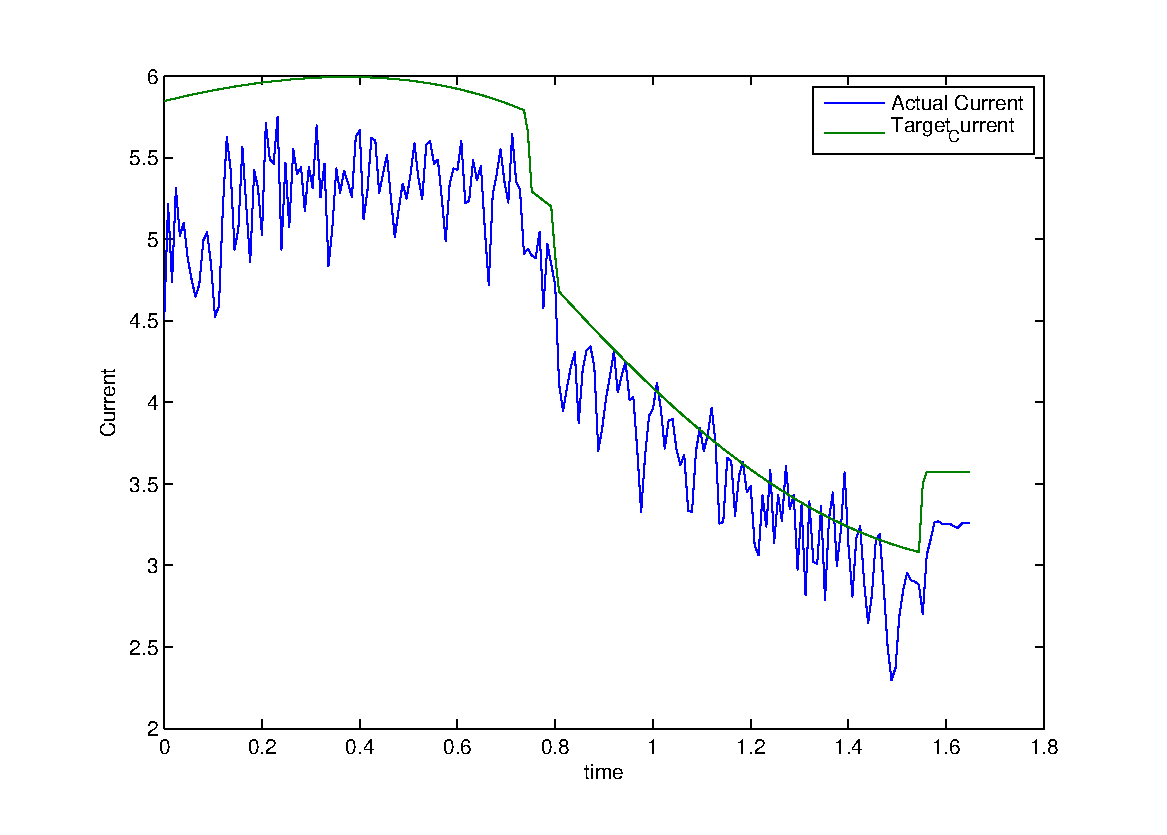
\includegraphics[width=1\textwidth]{pic/joint1_polyscope_current.eps}
      \caption[Soll und Ist-Werte der Stromstärke wärend der Bewegung des 2.Gelenks mit Polyscope]{Abbildung zeigt eindeutig den Berechneten Offset des Ist-Wertes.}
      \label{fig:current_profile_joint1_rci}
\end{figure}

\begin{figure}[H]
  \centering
    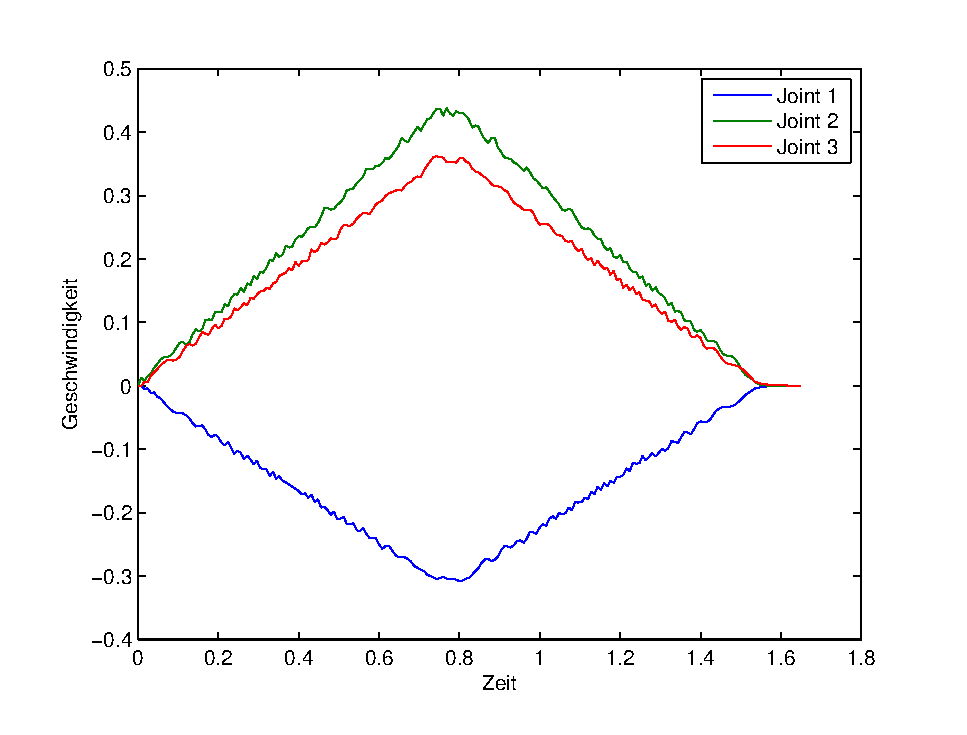
\includegraphics[width=1\textwidth]{pic/velocity_profile_polyscope.eps}
      \caption[Geschwindigkeitsprofil wärend der Bewegung der Gelenke 1-3 mit Polyscope]{Abbildung zeigt das Geschwindigkeitsprofil der Gelenke 1-3 wärend eines Bewegungsprofils mit Polyscope. Profil wurde mit der Echtzeitschnittstelle geloggt}
      \label{fig:velocity_joints_rci}
\end{figure}

\begin{figure}[H]
  \centering
    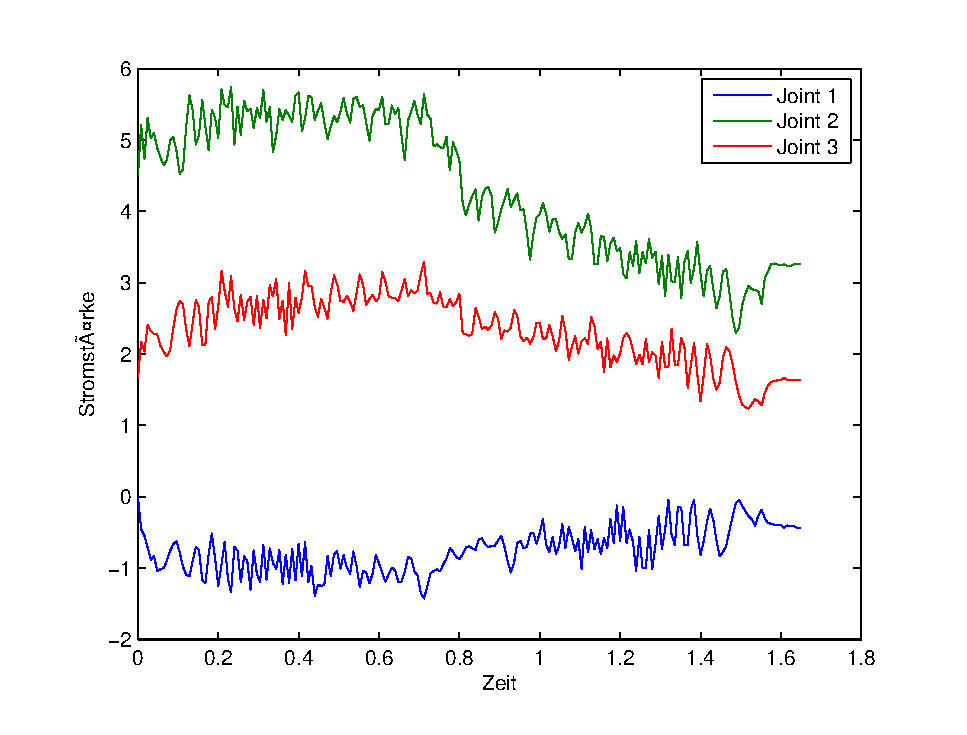
\includegraphics[width=1\textwidth]{pic/current_profile_polyscope.eps}
      \caption[Stromstärke wärend der Bewegung der Gelenke 1-3 mit Polyscope]{Abbildung zeigt die Stromstärke der drei Gelenke 1,2 und 3 wärend eines Bewegungsprofils. Profil wurde mit der Echtzeitschnittstelle geloggt}
      \label{fig:acceleration_profile_rci}
\end{figure}

\begin{figure}[H]
  \centering
    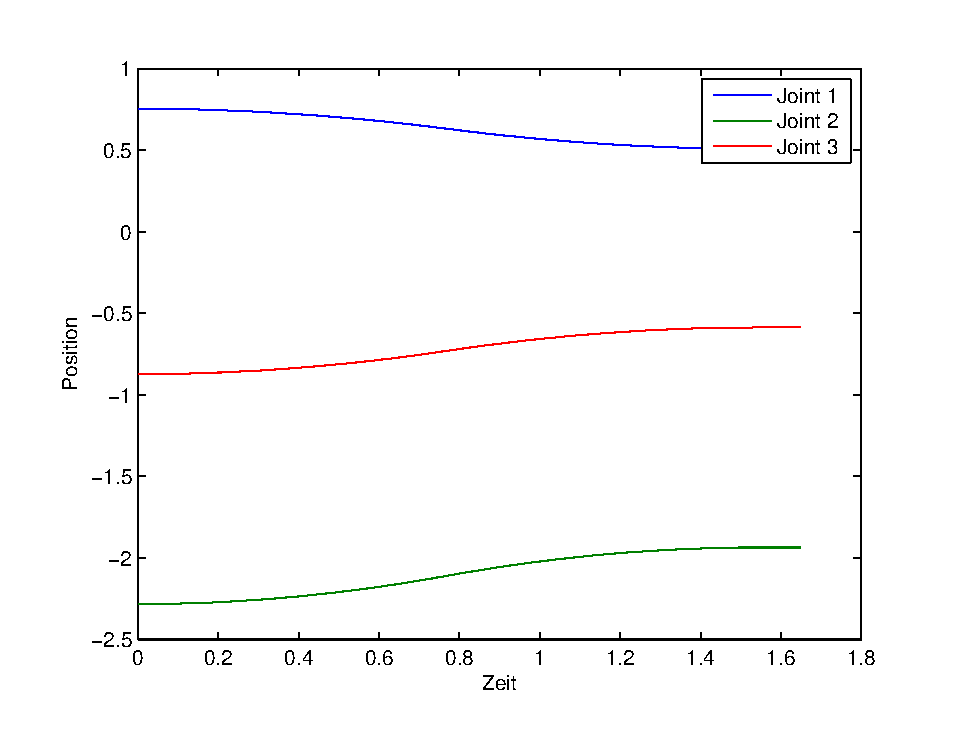
\includegraphics[width=1\textwidth]{pic/position_profile_polyscope.eps}
      \caption[Position wärend der Bewegung der Gelenke 1-3 mit Polyscope]{Abbildung zeigt die Position der Gelenke 1-3 wärend eines Bewegungsprofils mit Polyscope. Profil wurde mit der Echtzeitschnittstelle geloggt}
      \label{fig:position_joints_rci}
\end{figure}

\section{Bewegungsprofile geloggt in der C-\ac{API}}
\label{sec:profiles_with_capi}

\begin{figure}[H]
  \centering
    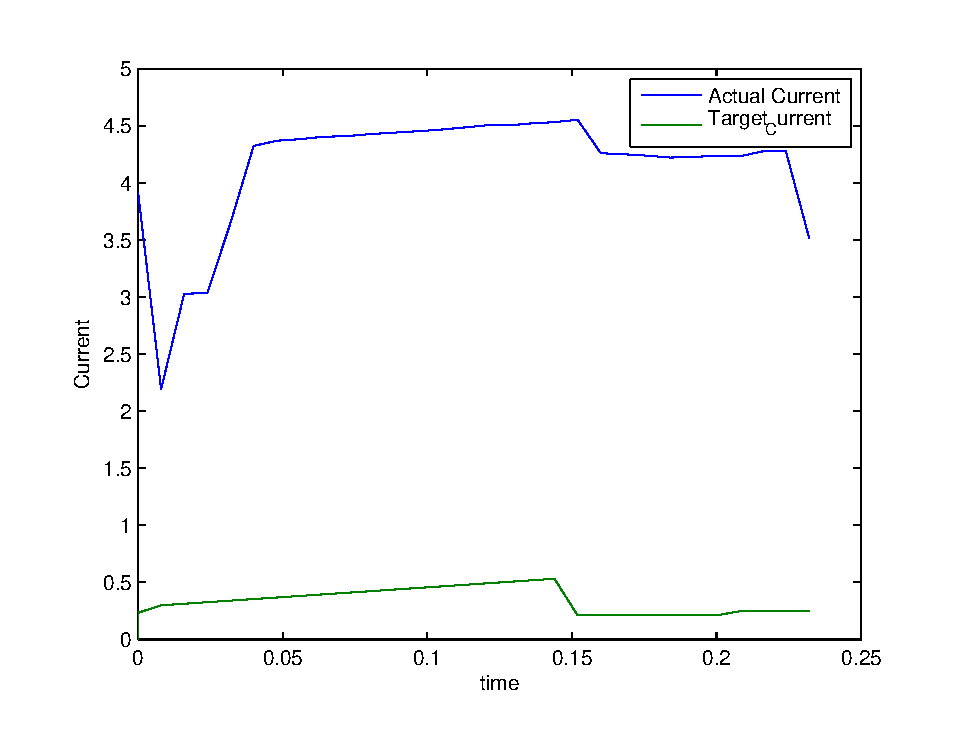
\includegraphics[width=1\textwidth]{pic/joint1_current_capi.eps}
      \caption[Soll und Ist-Werte der Stromstärke des 2.Gelenks]{Abbildung zeigt die Soll-Werte und Ist-Werte der Stromstärke des 2.Gelenks, kurz vor dem Sicherheitsstopp}
      \label{fig:joint_1_position_capi}
\end{figure}

\section{Bilder vom Roboter}
\label{pic_of_robot}

\begin{figure}[H]
  \centering
    \includegraphics[width=1\textwidth]{pic/tablet.jpg}
      \caption[Soll und Ist Werte der Position des 2.Gelenks]{}
      \label{fig:joint_1_position_capi}
\end{figure}


\chapter{Quellcode}
\label{quellcode}

\section{Speichern der Daten über TCP in der Datenbank}
\label{save_data_tcp_code_gru}

\begin{lstlisting}
#!/usr/bin/env python2.7

from my_utils import connection, Player, get_ip
import socket
import signal
import sys
import os

class SaveDataInterface():
    def __init__(self, interface="localhost"):
        self.__run_flag=False
        self.interface = interface
        self.socket=socket.socket(socket.AF_INET, socket.SOCK_STREAM)
        ip = get_ip(interface)
        if ip is None:
            ip="127.0.0.1"
        else:
            ip = get_ip(interface)
        port = 8000
        self.socket.setsockopt(socket.SOL_SOCKET, socket.SO_REUSEADDR, 1)
        try:
            self.socket.bind((ip, port))
            print "server is listen on %s:%d" %(ip, port)
            self.socket.listen(1)
        except socket.error, e:
            print(e[0])
            self.socket.close()
            self.socket=None

    def run(self):
        self.__run_flag=True
        # print("starting send interface waiting for queue")
        while self.__run_flag:
            if self.socket is not None:
                conn, addr = self.socket.accept()
                conn.settimeout(2)
                print "client connected: {0}".format(addr)
                player=None
                while self.__run_flag:
                    msg = self.read_from_socket(conn)
                    if msg is not None:
                        if msg == "new_patient":
                            # print("wait for new patient name")
                            name = self.read_from_socket(conn)
                            player = connection.Player()
                            player.name = name.rstrip()
                            player.save()
                        elif msg == "load_patient":
                            print("wait for patient name")
                            name = self.read_from_socket(conn)
                            player = connection.Player.find_one({'name': name.rstrip()})
                            if player is not None:
                                print("send %s"%"1".encode('ascii'))
                                print("positions %s"%("(%s)"%player.start_pos[1:-1]).encode('ascii'))
                                conn.send("(1)".encode('ascii'))
                                conn.send(("(%s)"%player.start_pos[1:-1]).encode('ascii'))
                            else:
                                conn.send("(0)".encode('ascii'))
                        elif msg == "set_patient_data":
                            # print("wait for player data")
                            start_position = self.read_from_socket(conn)
                            player.start_pos=start_position.rstrip()
                        else:
                            print("recieved unknown command")
                    else:   
                        break
                conn.close()

        self.socket.close()
        return 0

    # This Function reads from the Socket conn the next msg checks for errors
    def read_from_socket(self, conn):
        msg = None
        while self.__run_flag:
            try:
                msg = conn.recv(1024)
            except socket.timeout, e:
                err = e.args[0]
                # this next if/else is a bit redundant, but illustrates how the
                # timeout exception is setup
                if err == 'timed out':
                    # print 'recv timed out, retry later'
                    continue
                else:
                    print e
                    msg=None
            except socket.error, e:
                print e
                msg=None
            else:
                if len(msg) == 0:
                    msg=None
                    break
                else:
                    print msg
                    break
        return msg


sdi = SaveDataInterface(interface="eth0")

sdi.run()
\end{lstlisting}

 
\end{document}